\newtoggle{withbonus} \toggletrue{withbonus} % set true to show bonus points in grade table
\lstset{style=Python}

% setting underlying course name (Grundlagenfach Mathematik, §-Unterricht, \ldots)
\newcommand{\mycourse}{Grundlagenfach Informatik}
% name of the class
\newcommand{\myclass}{2. Klassen}
% set date
\newcommand{\mydate}{18. Oktober 2024}

\title{\textbf{Bilder bearbeiten in Python}}
\author{Fachschaft Informatik\\
	\mycourse, \myclass}
\date{\mydate}
\maketitle
\thispagestyle{headandfoot}
\clearpage

\section*{Vorbereitung}
\begin{enumerate}
	\item Erstellen Sie auf Ihrem eigenen Rechner einen neuen Ordner \emoji{file-folder} mit dem Namen
	      \begin{center}
		      {\tt Bilder_Bearbeiten}.
	      \end{center}
	\item Laden Sie die Datei {\tt dateien.zip} von Moodle herunter, und zwar so, dass die Datei {\tt dateien.zip} in dem neu angelegten Ordner {\tt Bilder_Bearbeiten} abgespeichert ist.
	\item Die Datei {\tt dateien.zip} ist komprimiert und muss zuerst entpackt werden. Entpacken geht ganz einfach so:
	      \begin{description}
		      \item[Windows:] Rechtsklick auf {\tt dateien.zip} und dann {\tt Alle extrahieren}.
		      \item[macOS:] Doppelklick auf {\tt datein.zip}
	      \end{description}
	\item Öffnen Sie das Python-File {\tt bilder\_template.py} in {\tt spyder} oder {\tt vscodium}.
	\item In diesem Python-File {\tt bilder\_template.py} ist ein Gerüst / Vorlage zu allen nachfolgenden Aufgaben bereits gegeben (Template). Bitte lösen Sie die Aufgaben, indem Sie diese Vorlage Schritt für Schritt durch Ihren Python-Code ergänzen.
\end{enumerate}


\begin{questions}
	\section*{Schwarzweissbilder}
	\question{\textbf{Anzahl der schwarzen Pixel in einem gegeben Bild zählen}}

	Schreiben Sie eine Python-Funktion \lstinline|def count_black_pixels(filename)|, welche das ein Schwarzweissbild mit dem Dateinamen \lstinline|filename| als Argument erhält und die Anzahl der schwarzen Pixel in diesem Bild zählt und diese Anzahl mit \lstinline|return| zurück gibt. Betrachten Sie dazu unbedingt die Vorlage.

	\question{\textbf{Schwarzweissbild invertieren}}

	Schreiben Sie eine Python-Funktion \lstinline|def invert_black_white_image(filename)|, welche ein Schwarzweissbild mit dem Dateinamen \lstinline|filename| als Argument erhält und dieses Bild invertiert: Alle weissen Pixel (Pixel mit Wert $1$) sollen schwarz werden und alle schwarzen Pixel (Pixel mit Wert $0$) sollen weiss werden.

	Stellen Sie schliesslich das originale Bild und das invertierte Bild nebeneinander dar.

	\question{\textbf{Bild von zufällig gewählten (schwarzweiss) Pixeln}}

	Schreiben Sie eine Python-Funktion \lstinline|def random_black_white_image(width, height)|, welche ein Schwarzweissbild mit den gegebenen Dimensionen (Breite / Höhe) erzeugt.
	Jeder Pixel soll dabei zufällig entweder schwarz (0) oder weiss (1) gewählt werden. Der Aufruf
	\begin{center}
		\lstinline|random_black_white_image(400, 600)|
	\end{center}
	sollte dann beispielsweise ein Schwarzweissbild der Breite 400 Pixel und Höhe 600 Pixel generieren, wobei jeder Pixelwert (0 oder 1) zufällig gewählt wurde.

	\section*{Graustufenbilder}

	\question{\textbf{Graustufen invertieren}}

	Schreiben Sie eine Python-Funktion \lstinline|def invert_grayscale_image(filename)|, welche ein Graustufenbild (256 Stufen) mit dem Dateinamen \lstinline|filename| als Argument erhält und dieses Bild invertiert: Aus dem hellen (weissen) Pixel mit Wert 255 soll der dunkle (schwarze) Pixel mit Wert 0 werden, der dunkle Pixel mit Werte 1 soll zum hellen Pixel mit Wert 254 werden und so weiter.

	Stellen Sie das originale Bild und das invertierte Bild nebeneinander dar.

	\question{Nur 8 verschiedene Graustufen}

	Schreiben Sie eine Python-Funktion \lstinline|def only_8_shades_of_gray(filename)|, welche ein Graustufenbild (256 Stufen) mit dem Dateinamen \lstinline|filename| als Argument erhält und mit nur 8 (anstelle von 256) verschiedenen Graustufen darstellt: Die Pixel mit Werten in $\lrc{0, 1, 2, \ldots, 31}$ sollen alle durch den Graustufenwert $0$ (schwarz) dargestellt werden, die Pixel mit Werten in $\lrc{32,33,34,\ldots, 63}$ durch den Wert $32$ und so weiter. Es ergeben sich also 8 Gruppen (Mengen), welche je 32 verschiedene Graustufenwerte durch denselben Graustufenwert darstellen.

	Stellen Sie das originale Bild und das transformierte Bild nebeneinander dar.



	\section*{RGB-Bilder}
	\question{\textbf{Grünanteil erhöhen}}

	Schreiben Sie ein Python-Funktion \lstinline|def increase_green(filename)|, welche ein RGB-Bild mit dem Dateinamen \lstinline|filename| als Argument erhält und den Grünanteil dieses RGB-Bilds um 20 Prozent verstärkt / erhöht. Es ist kein Problem, wenn ein Wert bei der Erhöhung den Wert $255$ übersteigt: Die Image-Library interpretiert jeden Wert $\geq 255$ als $255$.

	Stellen Sie das originale Bild und das transformierte Bild nebeneinander dar.

	(Bei Bildern mit Grünanteil von $> 212$ wird die Erhöhung natürlich de facto weniger als 20 Prozent betragen.)


	\question{\textbf{Sepia-Filter}}

	In dieser Aufgabe wollen wir einen Sepia-Filter (Sepia-Effekt) erstellen. Wie dieser Filter definiert ist, können Sie unter \url{https://de.wikipedia.org/wiki/Sepia_(Fotografie)} nachlesen. Der Sepia-Filter findet häufige Anwendung in den sozialen Medien (e.g. Instagram).

	Schreiben Sie ein Python-Funktion \lstinline|def sepia_filter(filename)|, welche ein RGB-Bild mit dem Dateinamen \lstinline|filename| als Argument erhält und den Sepia-Effekt auf das Bild anwendet.

	Stellen Sie das originale Bild und das transformierte Bild nebeneinander dar.


	\section*{Weitere Aufgaben}

	\question{\textbf{Vertikale Streifen}}

	Schreiben Sie ein Python-Funktion \lstinline|def vertical_stripes(filename)|, welche ein Graustufenbild mit dem Dateinamen \lstinline|filename| als Argument erhält. Die Funktion soll \enquote{vertikale Streifen} in gleichmässigen Abständen durch das Bild legen. Ein Beispiel dieser Transformation ist in \cref{fig:streifen} gegeben. Hier haben wir vertikale Streifen mit einer Breite von 2 Pixeln gewählt. Der Abstand (Anfang zu Anfang) der Streifen ist 7 Pixel (also 5 unveränderte Pixel zwischen Ende eines Streifens und dem Anfang des nächsten Streifens).
	\begin{figure}[H]
		\centering
		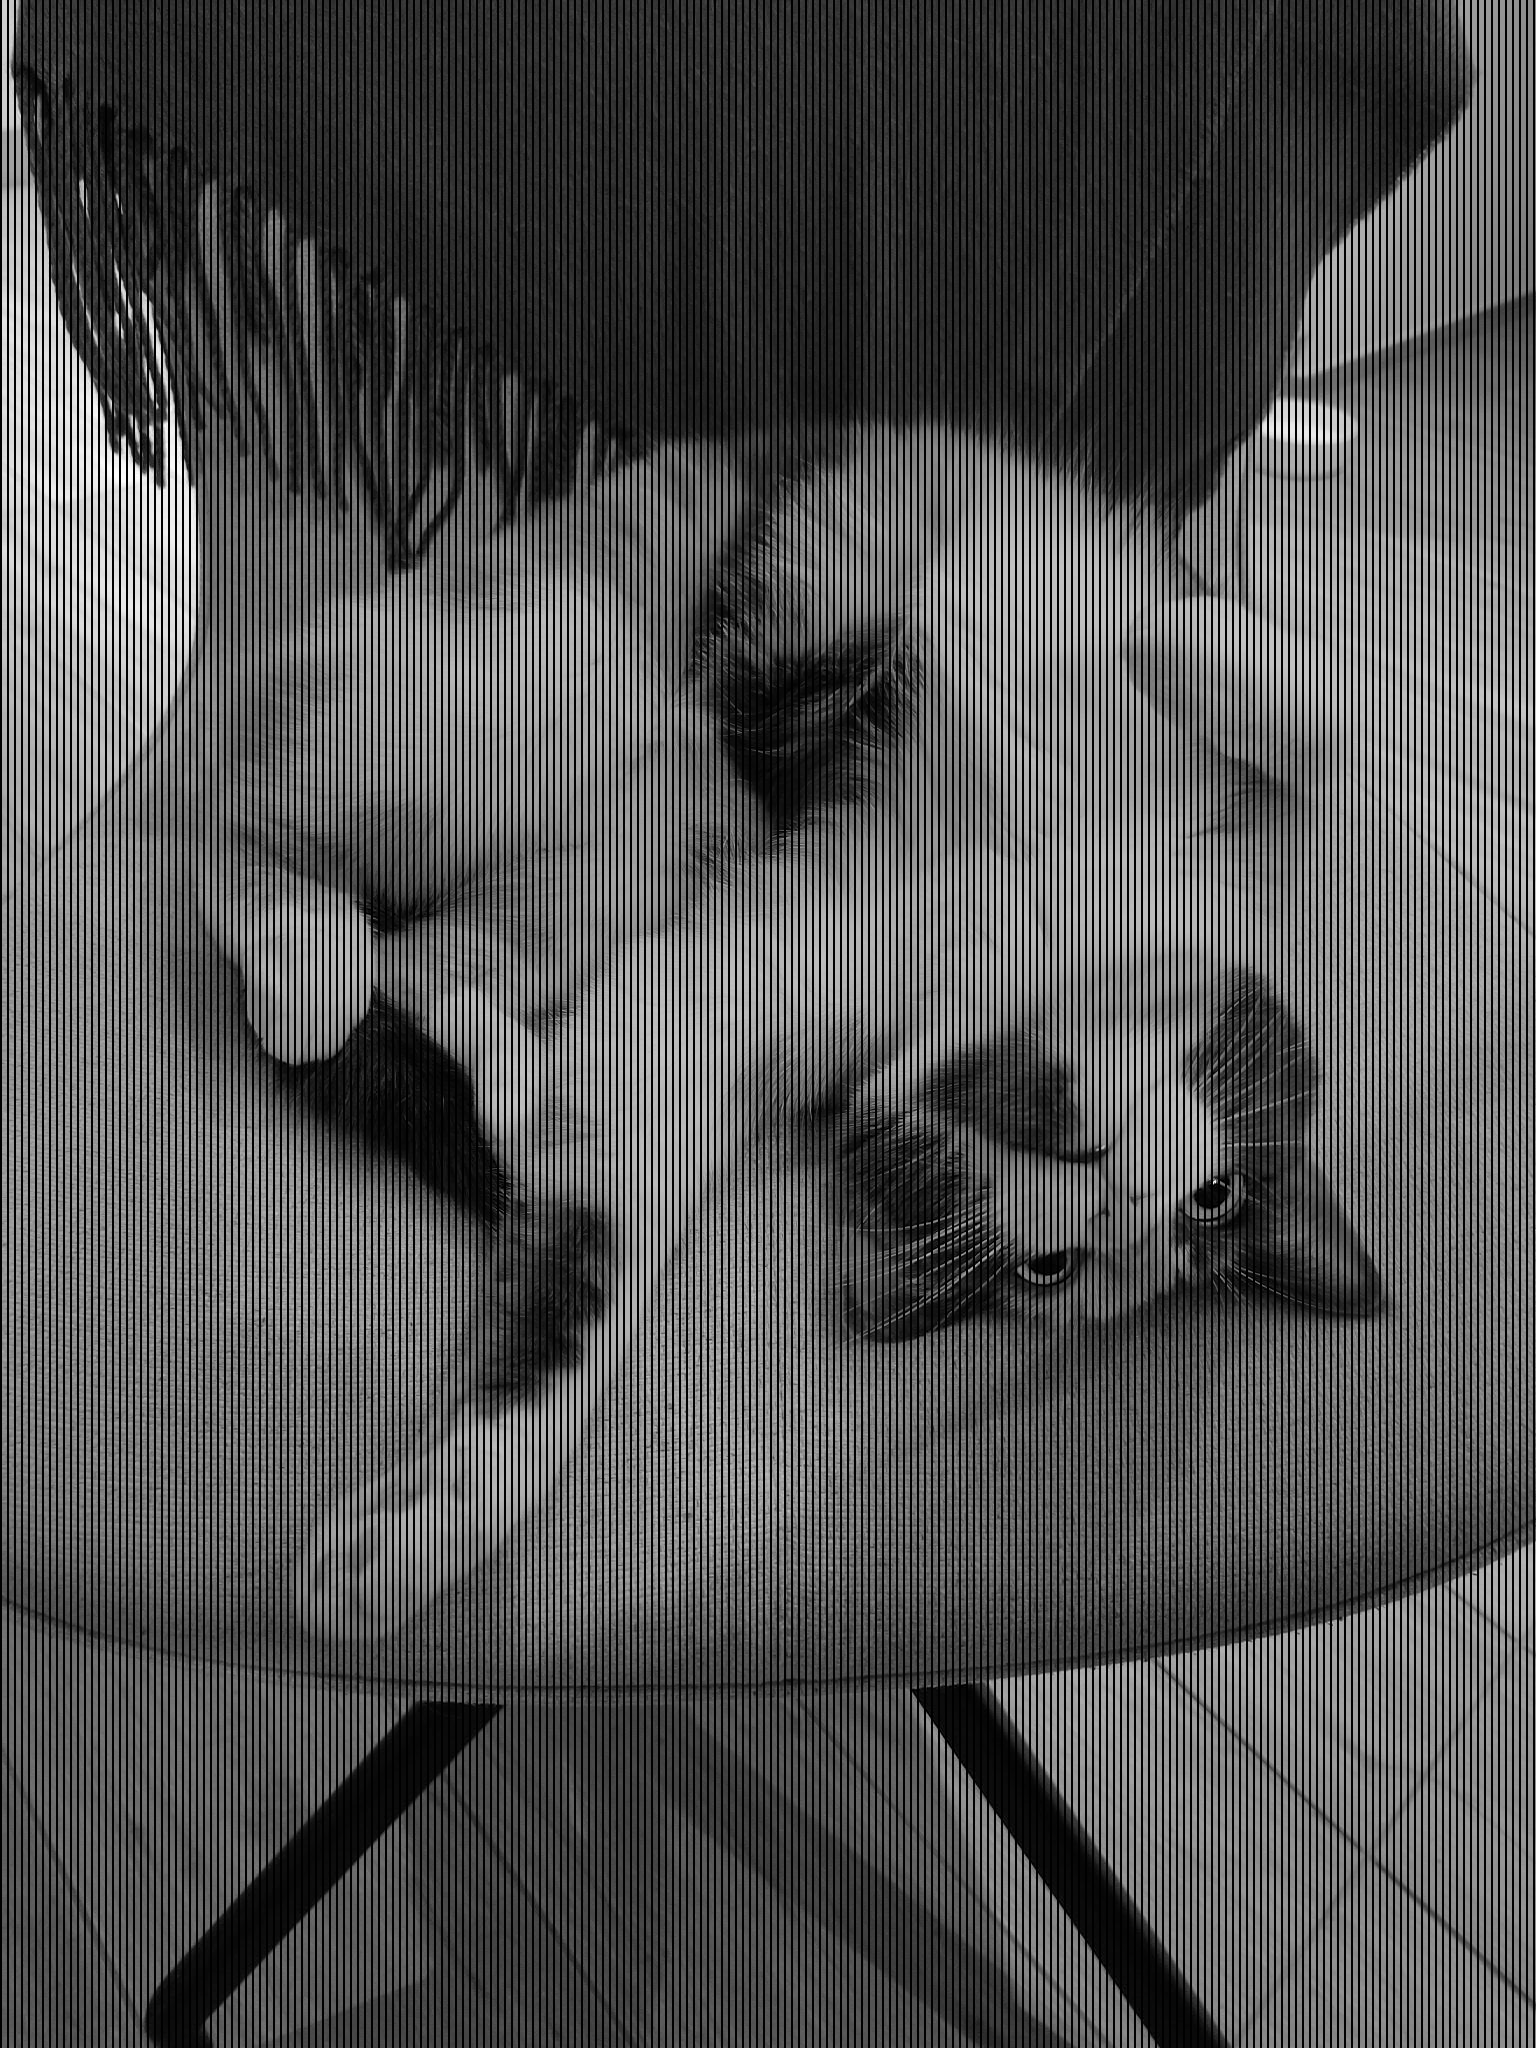
\includegraphics[width=0.5\textwidth]{Grundlagen_Info/00_Programmieren/Bilder_Bearbeiten/Vertikale_Streifen.PNG}
		\caption{Vertikale Streifen}
		\label{fig:streifen}
	\end{figure}

	\question{\textbf{Primzahlen als Pixel}}

	Schreiben Sie eine Python-Funktion \lstinline|def is_prime(number)|, welche für eine gegebene natürliche Zahl \lstinline|number| entscheidet, ob \lstinline|number| eine Primzahl ist (\lstinline|return True|) oder nicht (\lstinline|return False|).

	\begin{lstlisting}[language=Python,numbers=none]
        Testfälle:

        is_prime(0) # return False
        is_prime(23) # return True
        is_prime(97) # return True
        is_prime(91) # return False
	\end{lstlisting}

	Erstellen Sie nun eine leere Liste. Diese Liste soll am Ende ein Schwarzweissbild von $200\times 200$ Pixeln kodieren und somit eine Länge von $40000$ haben. Der $k$-te Eintrag der Liste für
	\begin{align*}
		k \in\lrc{0, 1, 2, \ldots, 39999}
	\end{align*}
	soll $0$ (schwarz) sein, falls $k$ eine Primzahl ist und $1$ (weiss) sonst.
\end{questions}
